% Chapter 2
\setlength\topmargin{8mm}
\onehalfspacing
\chapter{Principis de funcionament} % Main chapter title

\label{Chapter2} % For referencing the chapter elsewhere, use \ref{Chapter1} 

\rhead[\emph{Disseny, programació i implementació d'un robot de dibuix amb Arduino}]{\thepage}
\lhead[\thepage]{\emph{Disseny, programació i implementació d'un robot de dibuix amb Arduino}}

%----------------------------------------------------------------------------------------



%----------------------------------------------------------------------------------------

Aquest capítol és una introducció al funcionament del robot. S'explicaran els trets principals per tal d'entendre quin és el procés que s'ha de seguir per tal d'aconseguir dibuixar. Més endavant s'explicarà com s'han realitzat totes les etapes del projecte i per què s'ha fet d'aquesta manera. 

L'objectiu d'aquest dispositiu és aconseguir traspassar un disseny tècnic o dibuix realitzat per ordinador a la vida real sobre un paper. L'avantatge que presenta és que, al ser mòbil, a priori no té limitacions d'espai, pot fer-ho a l'escala que es desitgi mentre sigui sobre una superifície plana. El primer pas serà definir quins elements consituiran el robot i faràn possible aquest moviment. 

El robot presenta dues rodes motrius accionades per dos motors pas a pas que s'encarreguen de realitzar un moviment controlat i precís. Aquests estaràn controlats per un driver que actua com a etapa de potència i facilitarà el seu control, ja que funciona a partir de només 2 pins digitals, l'un controlador de l'step i l'altre de la direcció. Per tal de fer possible el moviment vertical del retolador s'utilitzarà un microservo que accionarà un mecansime per convertir la seva rotació en el moviment vertical del retolador dins una guia. Tot el conjunt estarà controlat per un microcontrolador Arduino UNO que es comunicarà amb l'ordinador mitjaçant una connexió Bluetooth. Tot el circuit s'alimentarà amb una bateria LiPo de 10000 mha amb dues sortides de 5V i d'1 i 2 A respectivament. Aquesta conexió es representa al següent diagrama:

\begin{figure}[H]
	\centering
	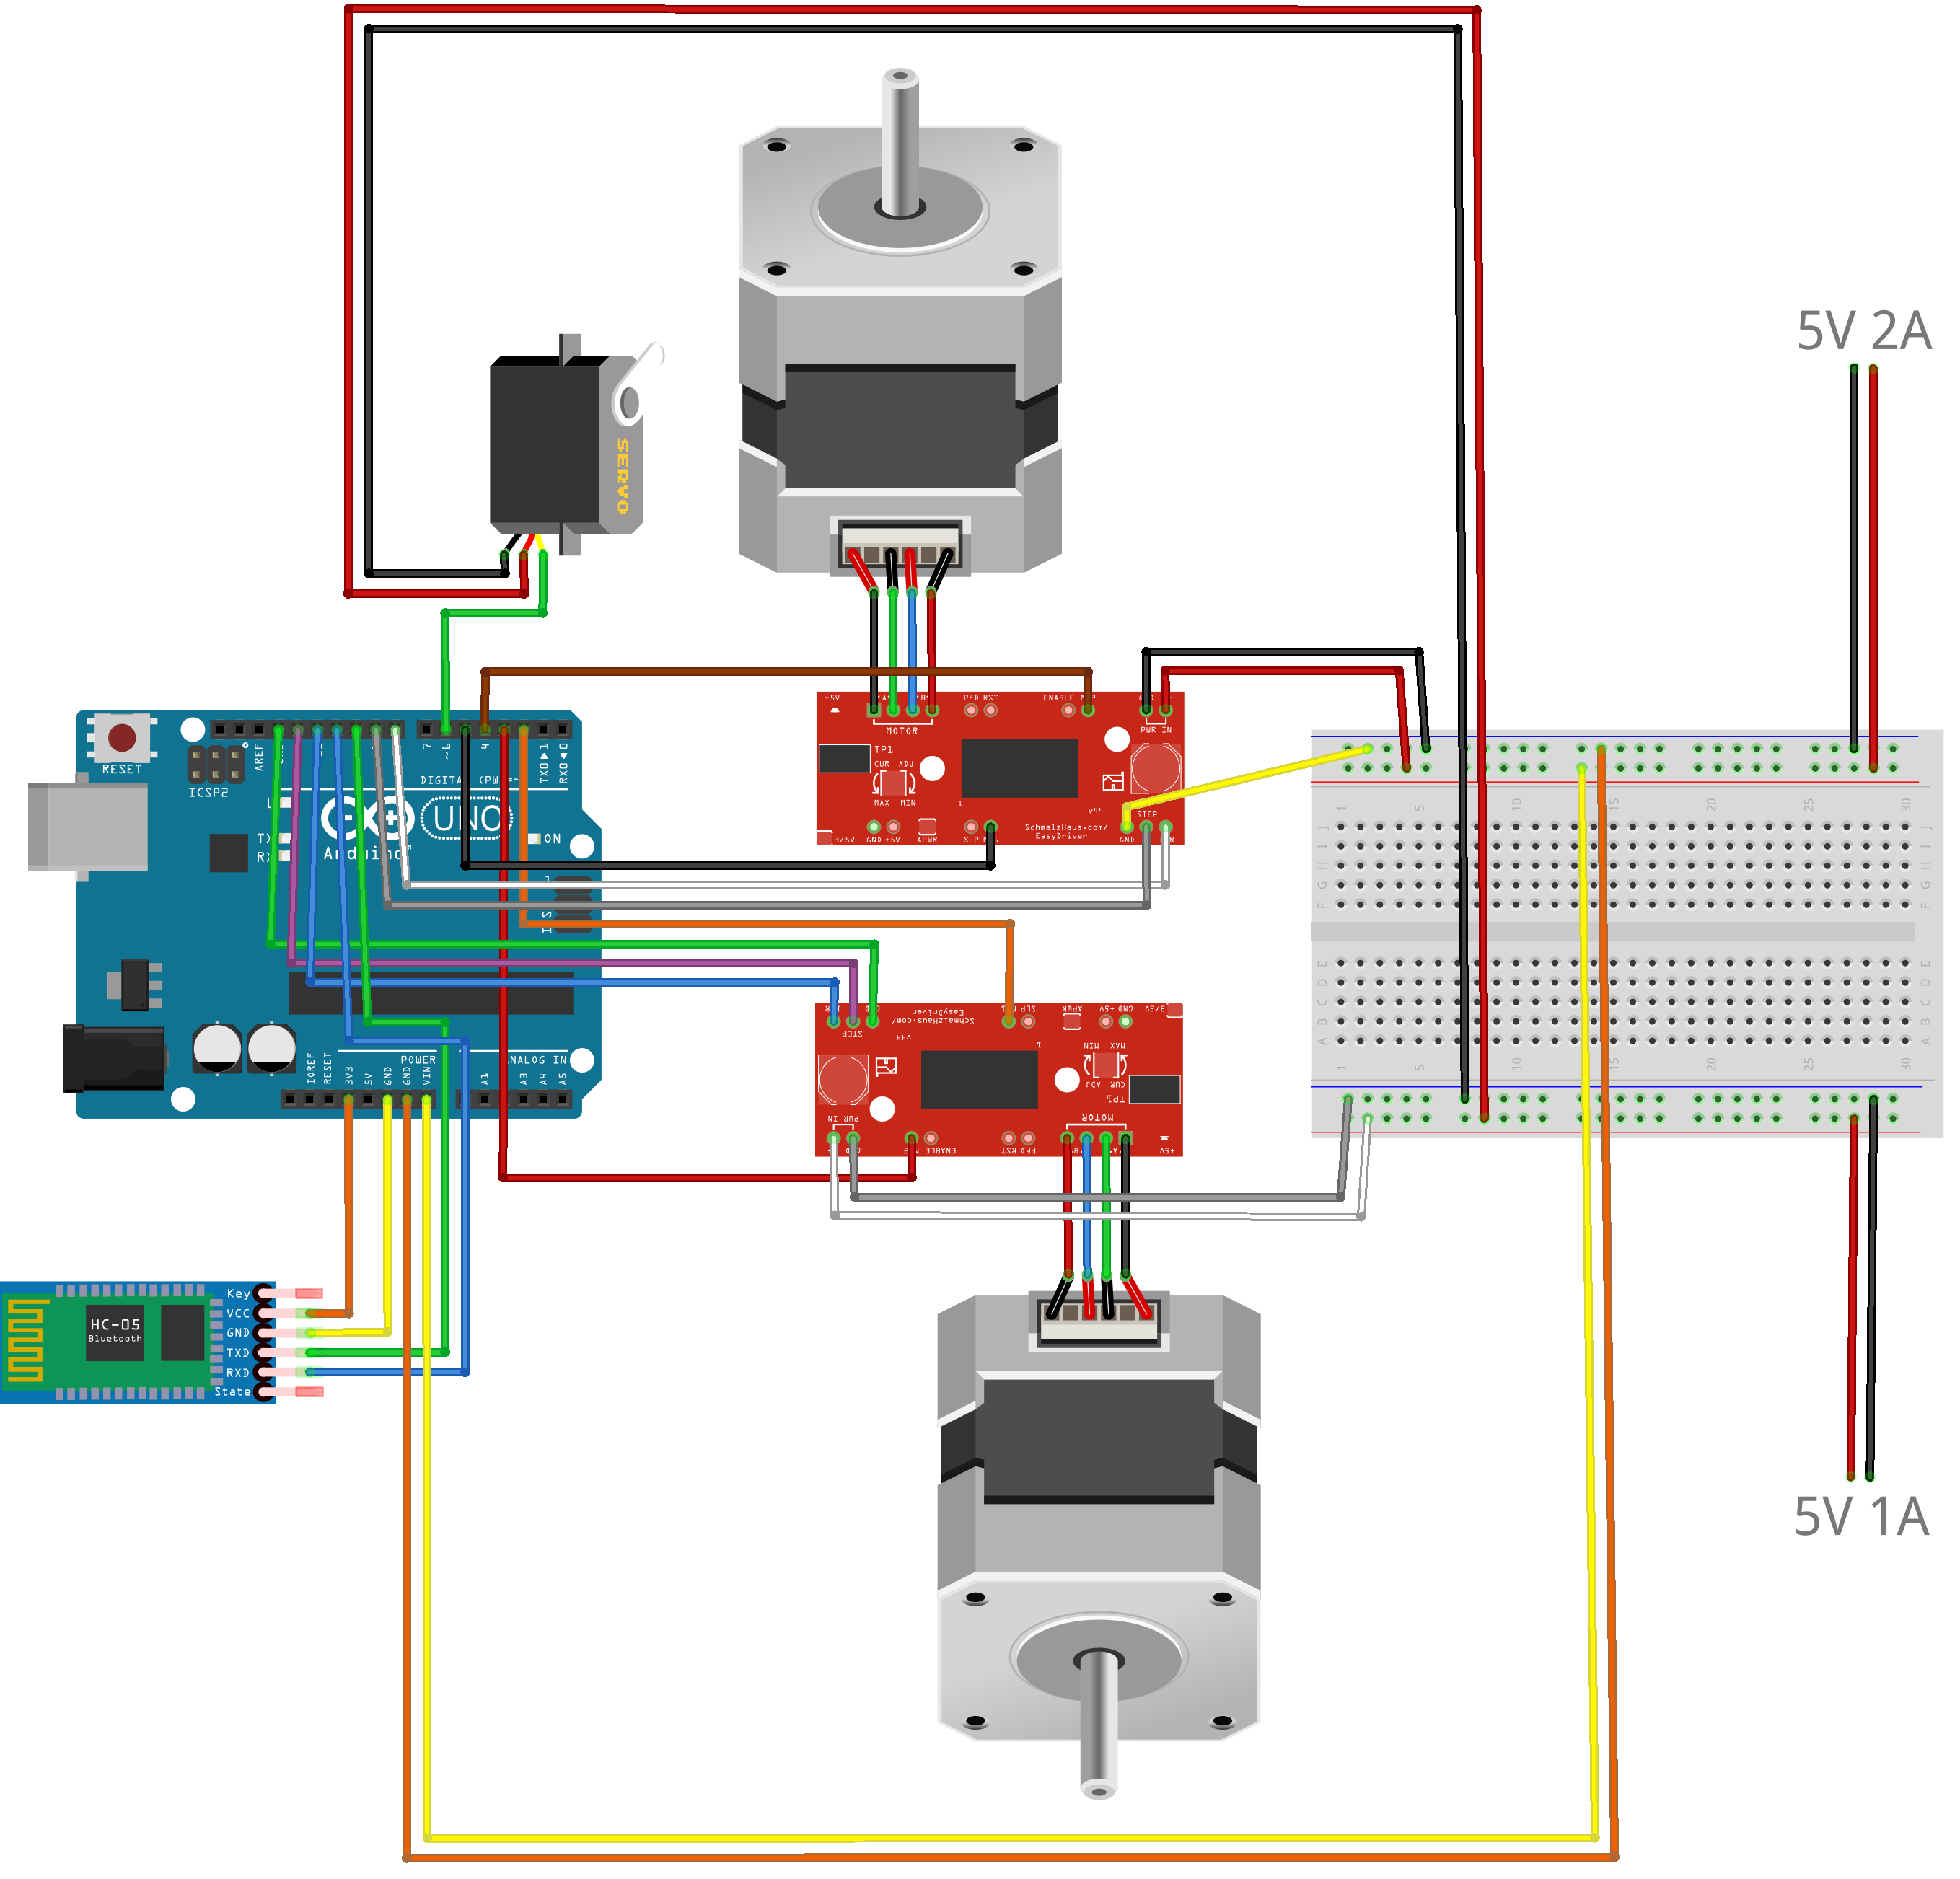
\includegraphics[scale=0.4]{RobotFritz}
	\caption{Diagrama de connexió dels components realitzada amb el programa Fritzing \cite{FritzingBib}.}
	\label{fig:connexio1}
\end{figure}

Un cop escollits els elements que formaran el robot s'haurà de dissenyar una estructura que incorpori tots aquests i permeti al robot fer la seva funció, intentant sempre optimitzar el tamany per fer-lo el més petit possible. Caldrà dissenyar diferents peces: un xassís, les rodes, una roda davantera i un mecanisme capaç de realitzar el moviment vertical del retolador. Aixó es realitzarà a partir de SolidWorks i s'imprimirà en 3D a l'aula Rep Rap de l'escola. 

\begin{figure}[H]
	\centering
	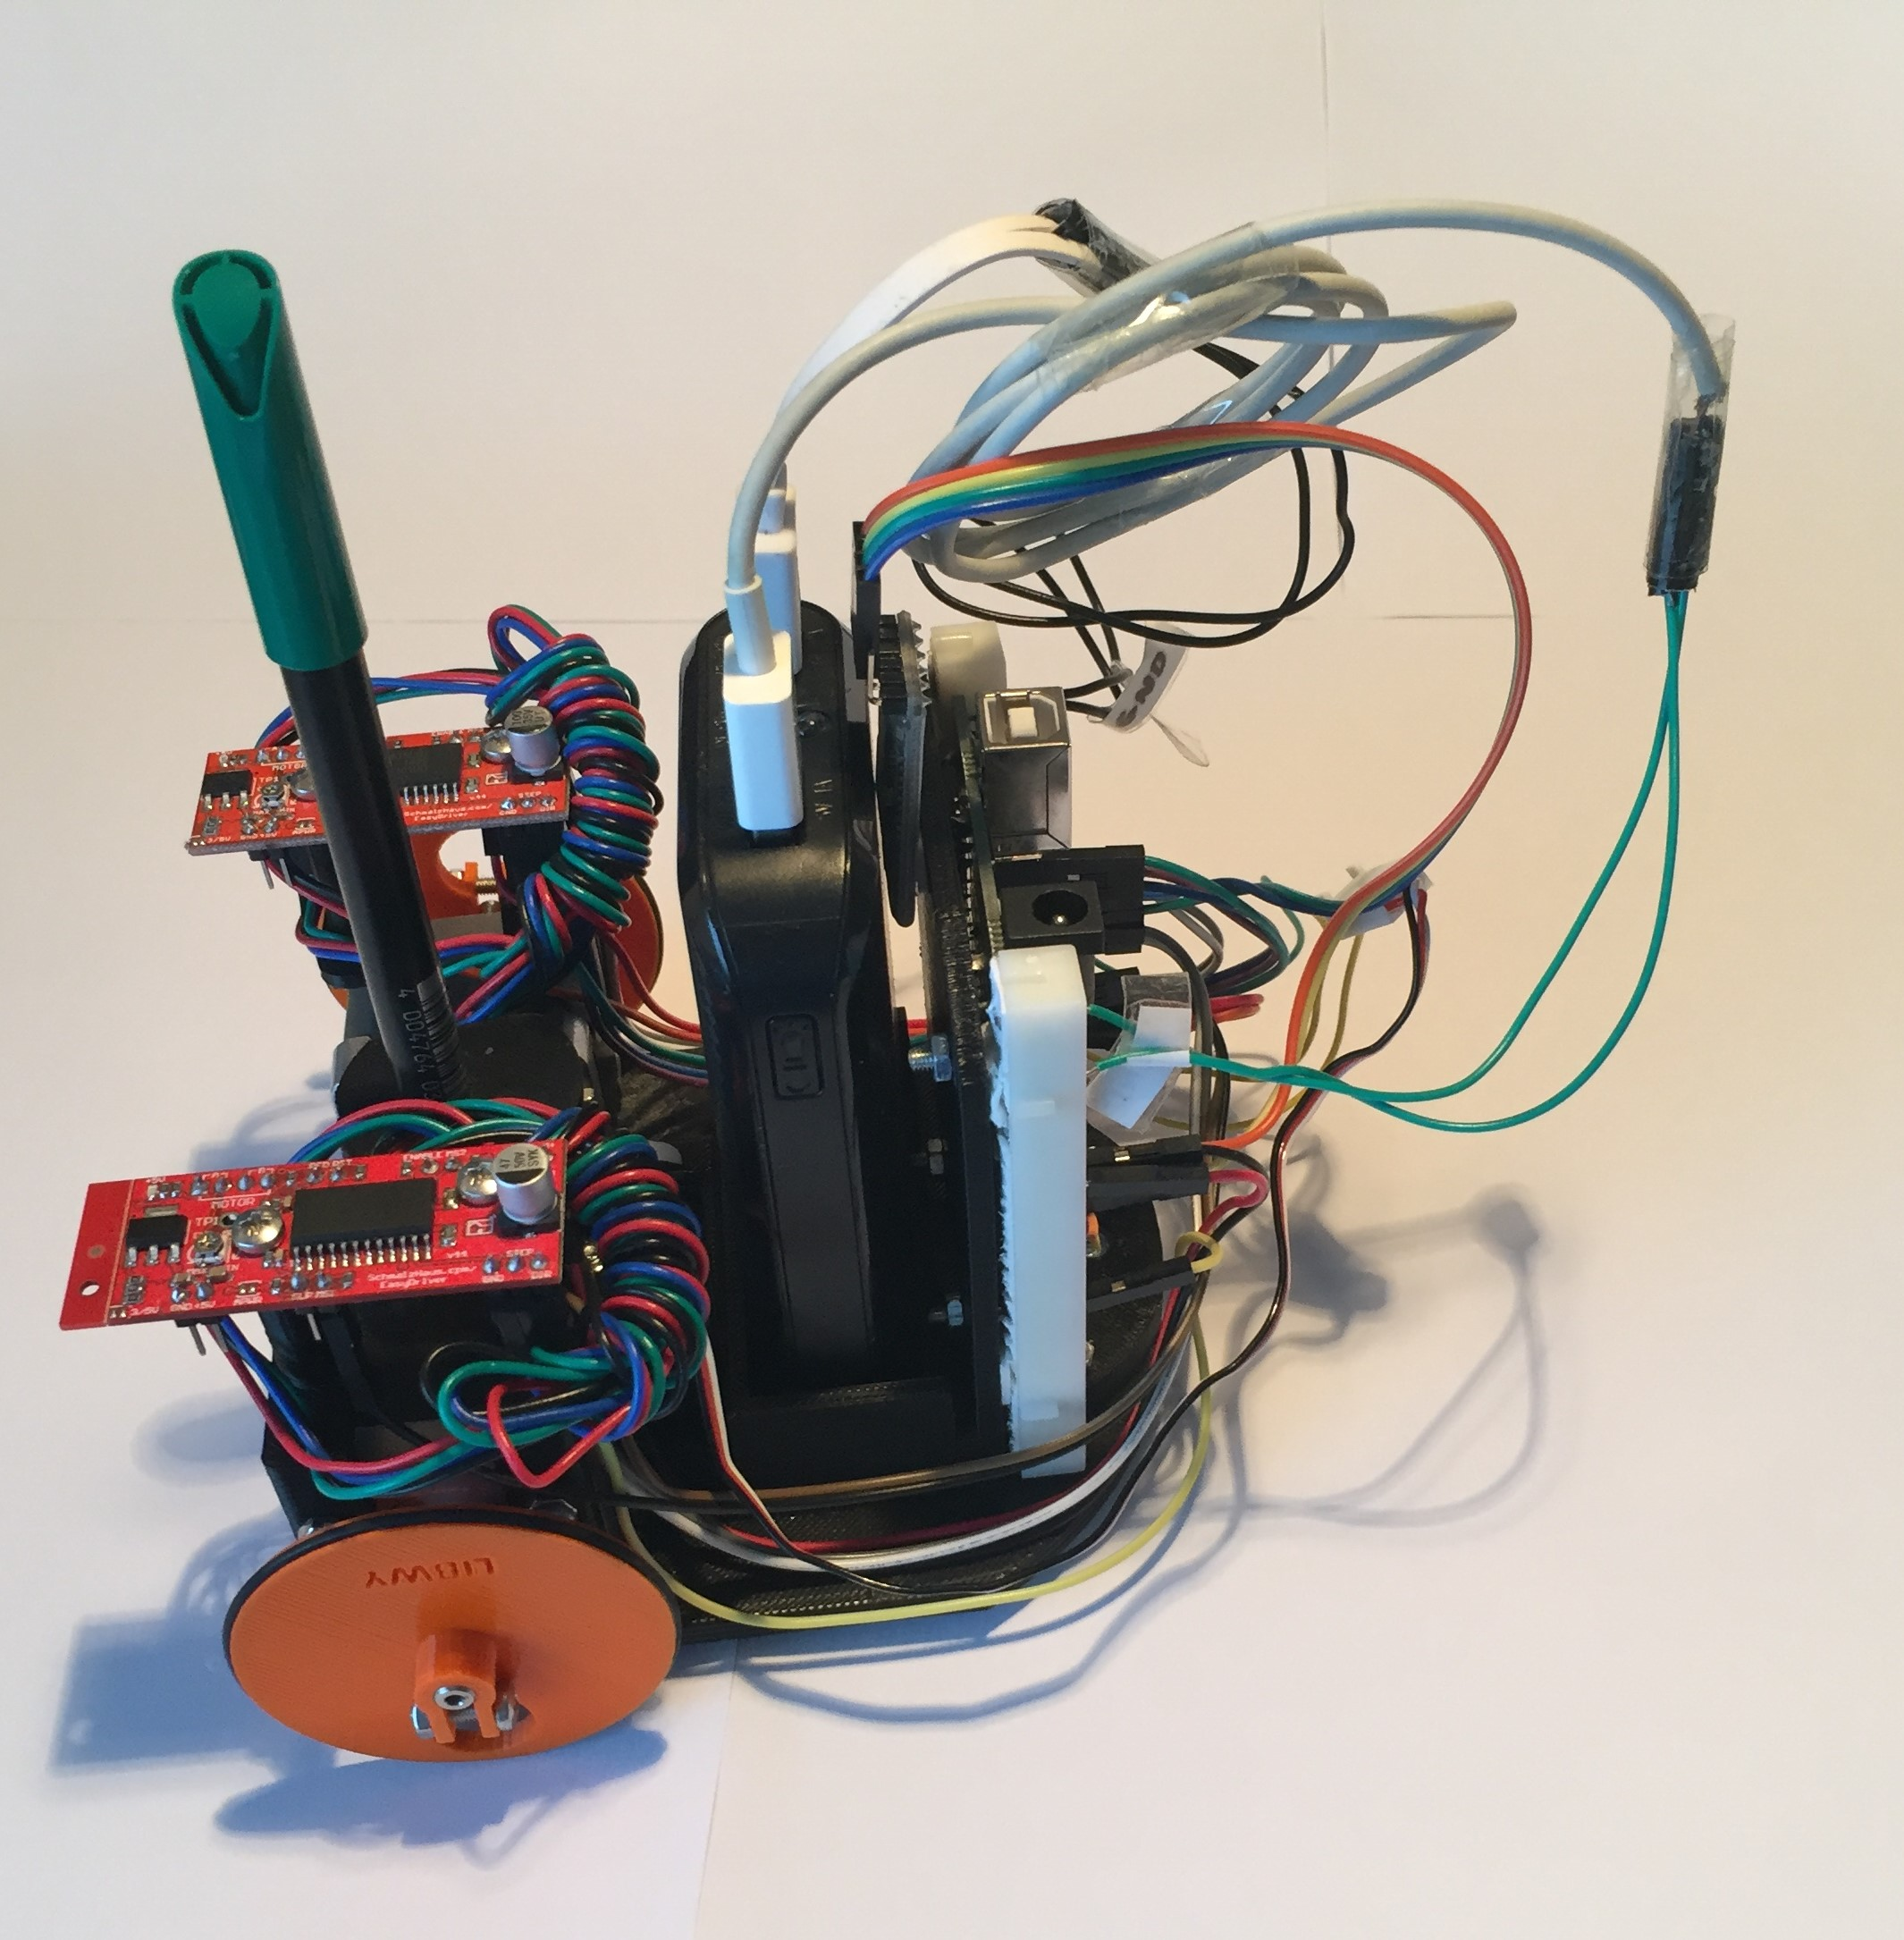
\includegraphics[scale=0.1]{RobotFoto}
	\caption{Fotografia del robot.}
	\label{fig:foto}
\end{figure}

Per últim caldrà crear el software controlador del robot. Des de l'ordinador, es processarà la imatge i s'extreuàa el GCode de la trajectòria, d'aquest GCode s'extreuran les ordres de moviment i es traduiran a passos del motor, que s'enviaran a l'Arduino per una connexió Bluetooth i aquest s'encarregarà de moure els motors. 

\begin{figure}[H]
	\centering
	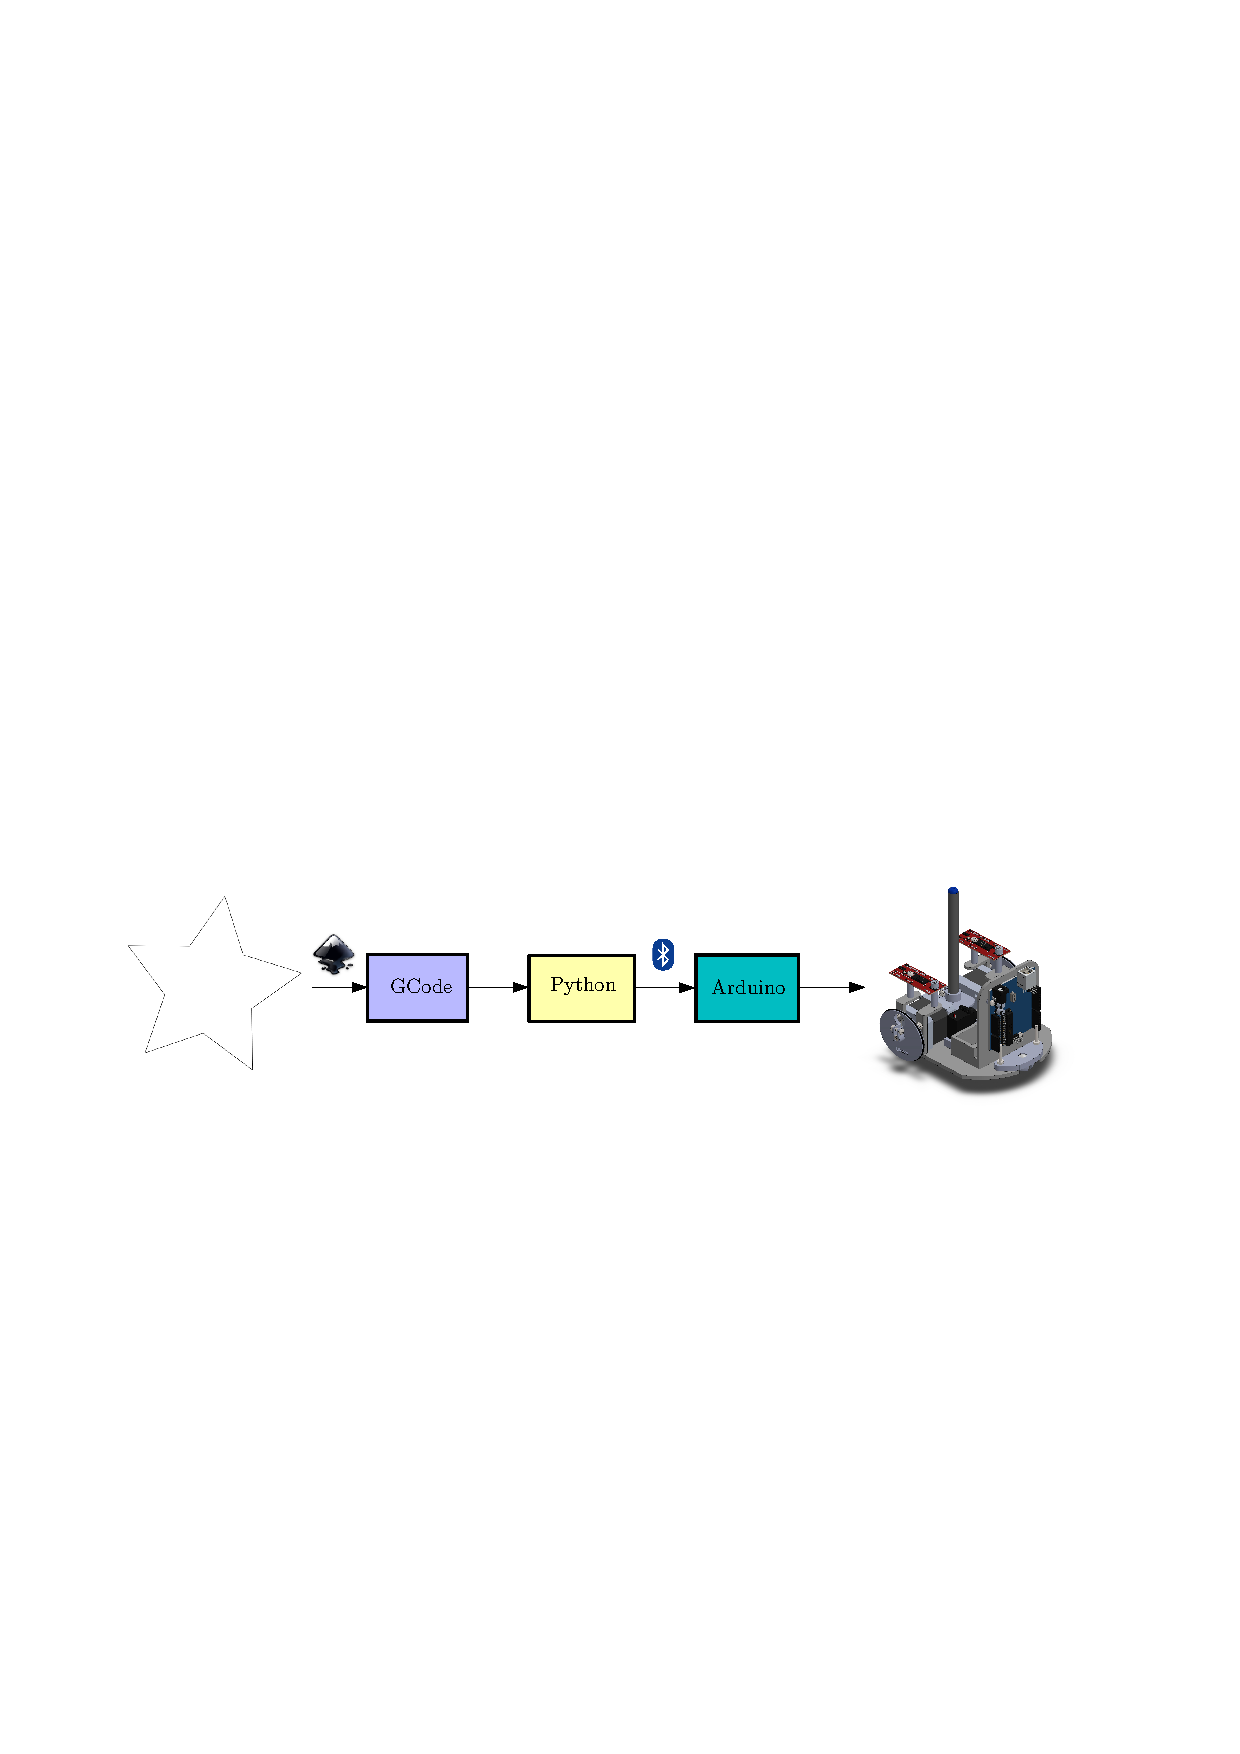
\includegraphics{Flux}
	\caption{Diagrama de flux del funcionament general.}
	\label{fig:flux}
\end{figure}

Aquest és el funcionament bàsic del robot i, a continuació, s'explicarà cadascuna de les parts de manera més detallada. 












